\section{The Front-end Electronics}
\subsection{Board layout}
The FEB64 \cite{Rodriguez:2015upa} is a 3U x 220 mm module (figure \ref{fig:FEB64}). A 19'' Eurocard chassis without backplane can accommodate up to 14 boards. Both front and rear ends are used for power and I/O. The front panel houses a 6-pin power connector, a JTAG connector to program the FPGA, a selectable HDMI (bottom) or RJ-45 (top) connector to the DAQ interface and 5 LEDs. The rear of the module houses the four (two on each side) connectors to the tracking plane, as described in sections \ref{sec:DB} and \ref{sec:ext}, as well as a 4-pin LEMO connector that brings the SiPM bias from a dedicated voltage source and forwards the remote temperature sensor wires to the same source for gain compensation \cite{Gil:2011cma}.

\begin{figure}[h!]
\centering
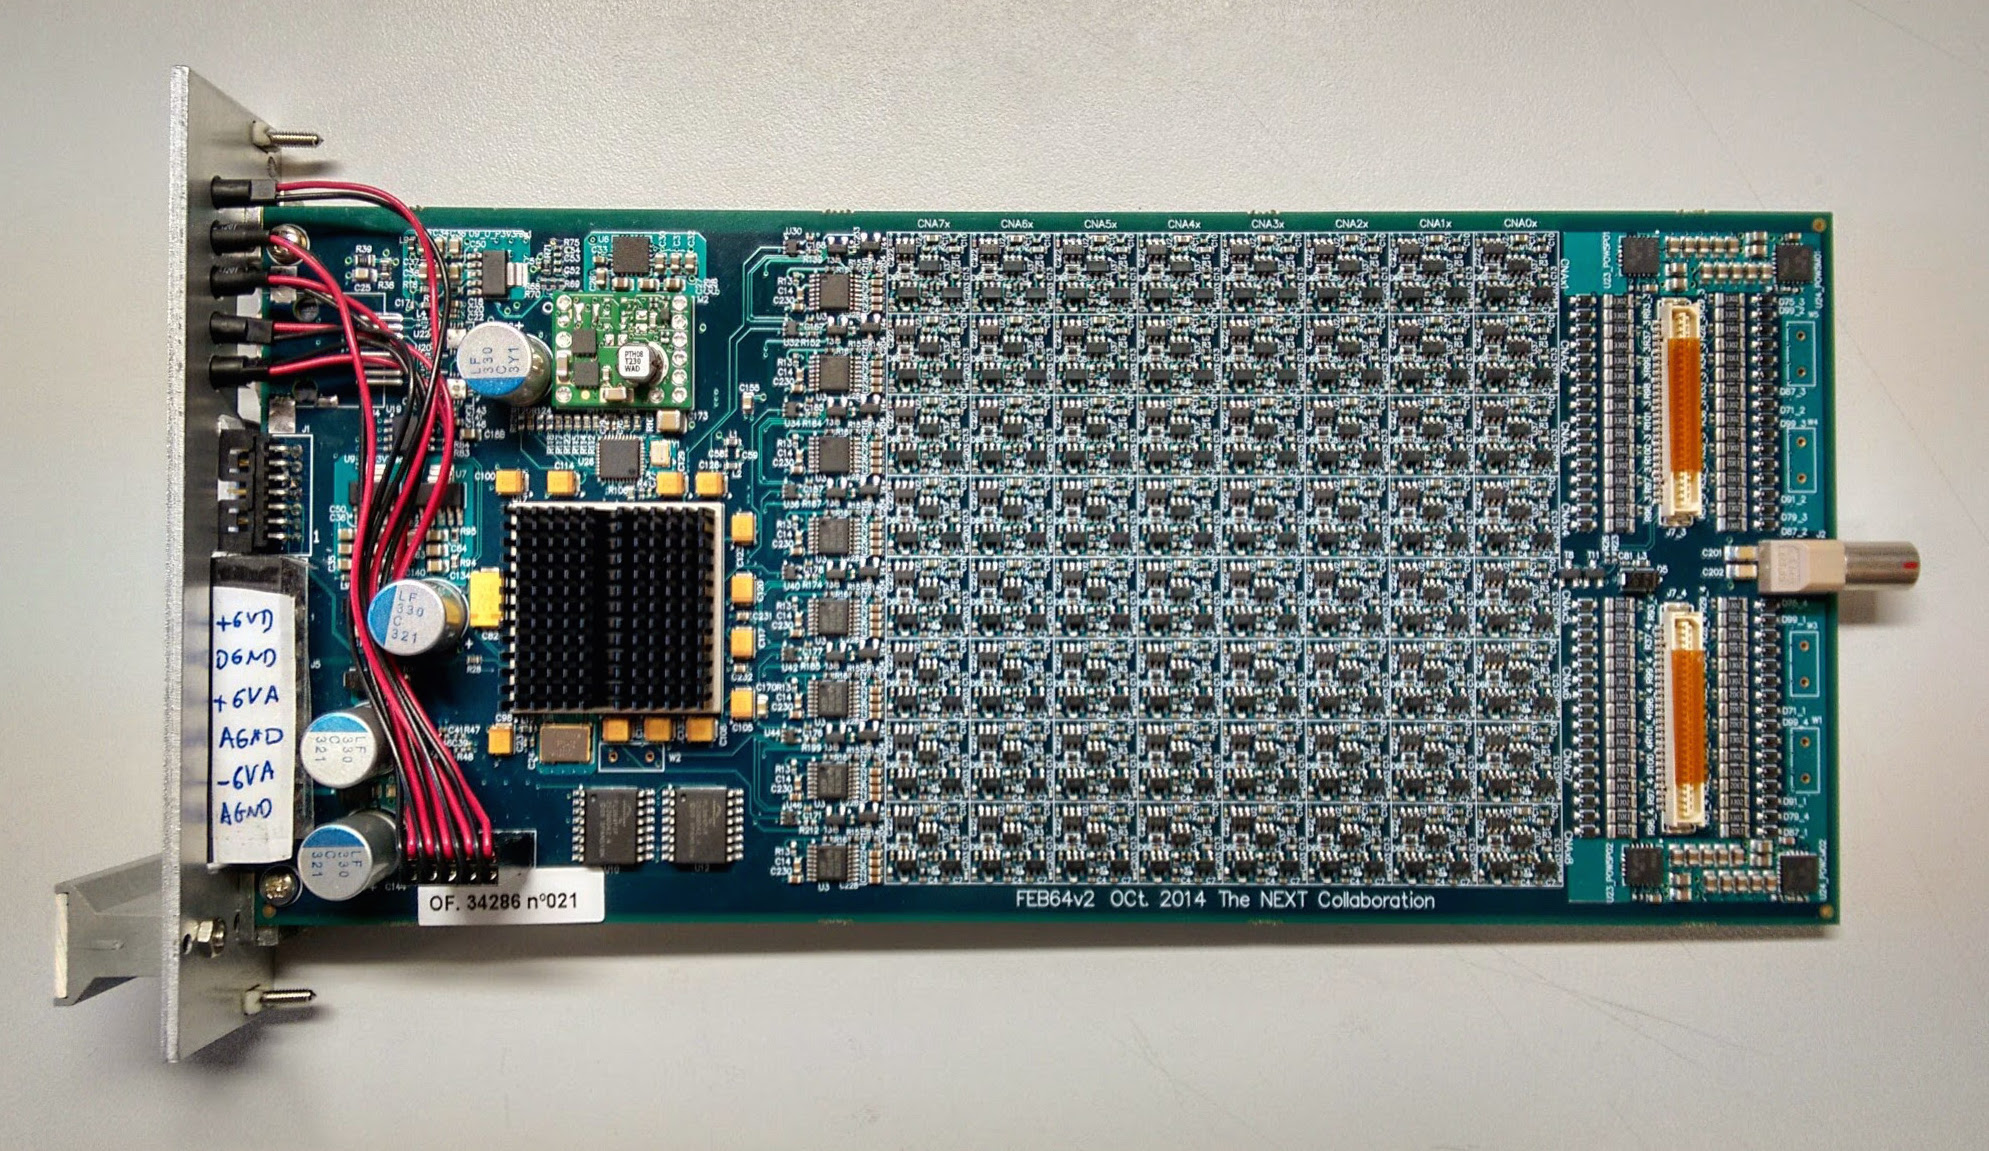
\includegraphics[width=.7\textwidth]{IMG/FEB64.JPG}
\caption{The FEB64 board.}
\label{fig:FEB64}
\end{figure}

The digital circuitry (FPGA, LVDS buffers, flash memories and voltage regulators for the digital ICs) reside on the left side of the card. The 64 analog channels (consisting each of two operational amplifiers, ADC and switch, as described in section \ref{sec:analog}) are located on the right side, in an 8-by-8 matrix. At the left of the matrix, a column with eight 8-channel DACs provide the voltages for the per-channel offset compensation.

\subsection{The analog section: amplification and integration}\label{sec:analog}
The SiPM is biased at the front end board. Anode and cathode lines run to the SiPM sensors in a balanced configuration, as described in sections \ref{sec:DB} and \ref{sec:ext}. Two resistors at the front-end input limit the current in the case of a SiPM short circuit and keep line balance.
A differential-input transimpedance amplifier based on the low-power low-cost AD8055 operational amplifier reduces common mode noise and amplifies the SiPM current by approximately 1400 with a 10-MHz bandwidth. A per-channel automatic offset voltage compensation is implemented thanks to the on-board FPGA, which reads the ADC values, calculates the baseline and provides a DC compensation voltage via a DAC at the input of the integrating stage.
The gated integrator, also based on the AD8055, provides the required gain (15 ADC counts per photoelectron, as the expected dynamic range is 250 photoelectrons in a microsecond and the ADC resolution is 12 bits). The switch is controlled by the FPGA at a 1 MHz rate. A few tens of nanoseconds are used to discharge the integrating capacitor, leaving the rest of the microsecond for integration.

\begin{figure}[h!]
\centering
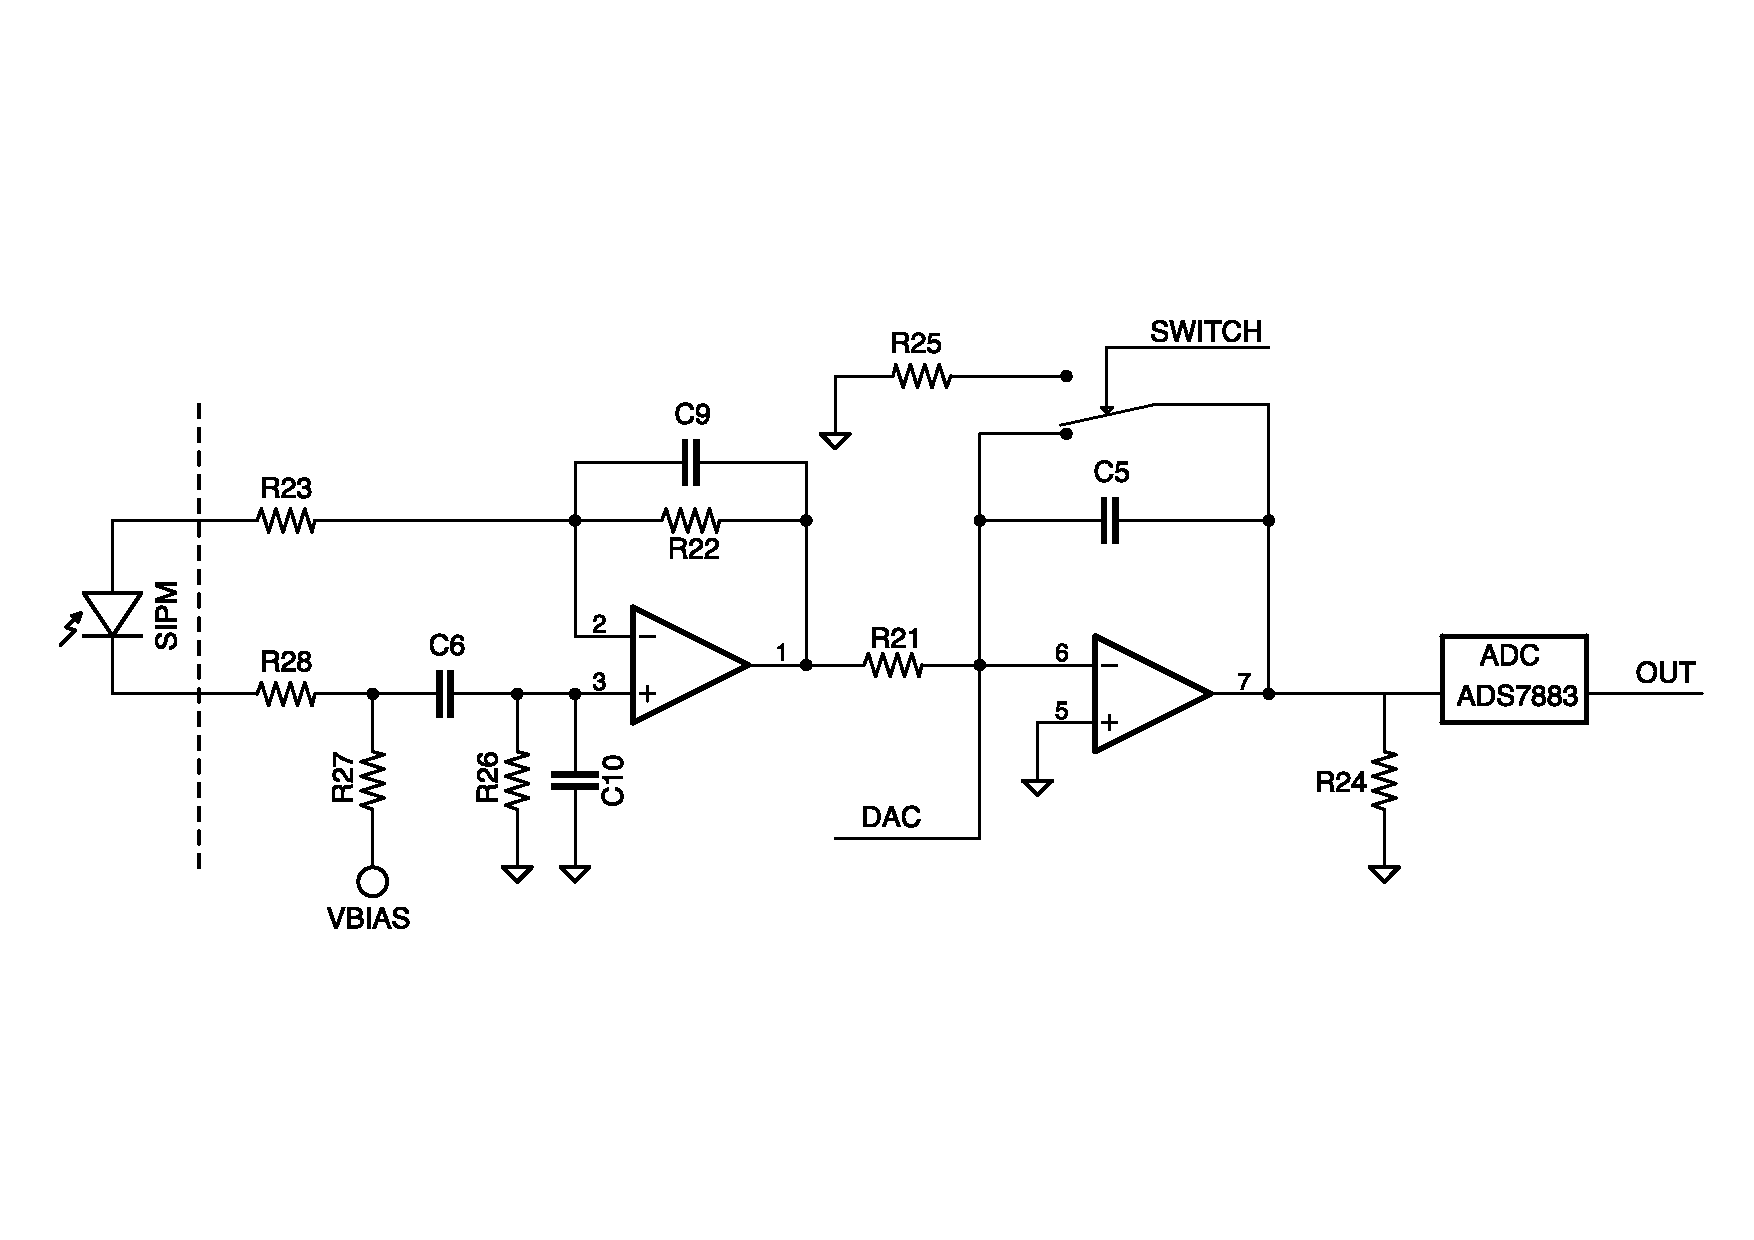
\includegraphics[width=.8\textwidth]{IMG/Analog.pdf}
\caption{The analog channel circuit.}
\label{fig:analog}
\end{figure}

Compared to the previous NEXT-DEMO front-end electronics \cite{Herrero:2012sa}, an amplification stage has been eliminated, the analog channel power (including the ADC) has been reduced to maximum 150 mW, a factor of 3.5, cost is one third, the number of channels per front-end board has been increased by a factor of 4 and a higher signal-to-noise ratio has been achieved thanks to the differential input stage. As a result, the FEB64 board is a valid solution for tracking planes in the scale of NEW and NEXT-100 (1800 and 7000 channels, respectively).


%%%%%%%%%%%%%%%%%%%